% Courtesy Leonard Wollenberg, 2024
% Compile with:
%    lualatex quark-model.tex
% then import the PDF with Inkscape and export as optimised SVG. Only internal import by Inkscape results in a small SVG file.
% Optionally, further compress the SVG with SVGO:
%    npm install -g svgo
%    svgo --multipass quark-model.svg
% With the newest version of Inkscape, you can also use the command line:
%    inkscape quark-model.pdf --export-plain-svg --export-type=svg --pages=1 --pdf-font-strategy=draw-missing
%    scour quark-model.svg new-quark-model.svg --enable-id-stripping --enable-comment-stripping --no-line-breaks --remove-descriptive-elements --set-precision=8 --shorten-ids
%    mv new-quark-model.svg quark-model.svg
%    svgo --multipass quark-model.svg

\documentclass{standalone}
\usepackage{tikz}
\usetikzlibrary{angles, arrows, arrows.meta, calc, decorations.pathmorphing, decorations.pathreplacing, decorations.shapes, positioning, quotes, shapes}
\usepackage{pgfplots}
\usepackage[compat=1.1.0]{tikz-feynman}
\usetikzlibrary{shadings}
\pgfplotsset{compat=1.18}


\begin{document}
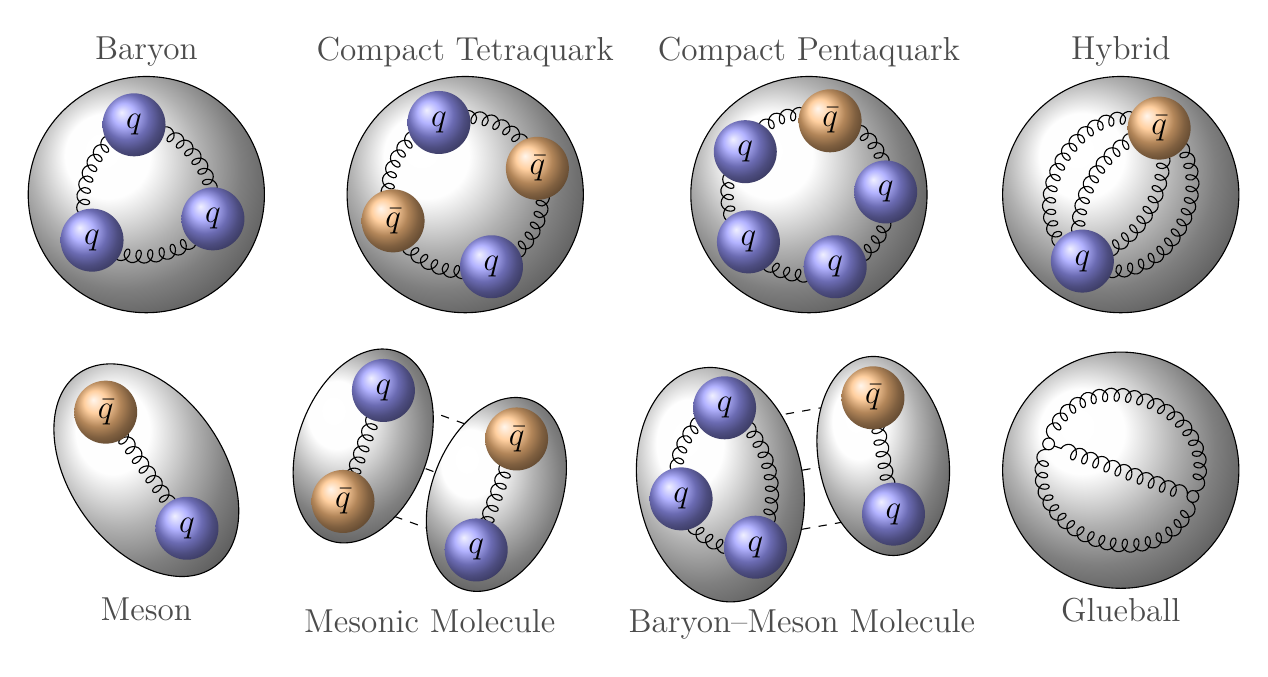
\begin{tikzpicture}
  \def\X{4.5}
  \def\Y{3.5}
  \def\QuarkRadius{0.4}
  \def\HadronRadius{1.5}
  \tikzset{every node/.style={font=\large}}

  \newcommand{\baryon}[1]{
    \shade[ball color=lightgray!2!white] (#1) circle (\HadronRadius);
    \draw[black] (#1) circle (\HadronRadius);
  }
  \newcommand{\meson}[1]{\ellipse{#1}{\HadronRadius}{0.65*\HadronRadius}}
  \newcommand{\smallbaryon}[1]{\ellipse{#1}{\HadronRadius}{0.7*\HadronRadius}}
  \newcommand{\smallmeson}[1]{\ellipse{#1}{0.85*\HadronRadius}{0.55*\HadronRadius}}
  \newcommand{\ellipse}[3]{
    \shade[ball color=lightgray!2!white] (#1) ellipse (#2 and #3);
    \draw[black] (#1) ellipse (#2 and #3);
  }

  \newcommand{\quark}[1]{\spherequark{#1}{\QuarkRadius}{$q$}{blue!40!white}}
  \newcommand{\antiquark}[1]{\spherequark{#1}{\QuarkRadius}{$\bar{q}$}{orange!50!white}}
  \newcommand{\spherequark}[4]{\shade[ball color=#4] (#1) circle (#2) node {#3}}

  \coordinate(center) at (-0.75*\X,0);
  \node[above=\HadronRadius of center, color=black!70] {Baryon};
  \baryon{center}
  \begin{scope}[rotate around={-20:(center)}]
    \def\nQuarks{3}
    \foreach \k in {1,...,\nQuarks}
    \coordinate[rotate around={(\k-1)*360/\nQuarks:(center)}] (q\k) at ($(center) + 0.6*(\HadronRadius,0)$);
  \end{scope}
  \begin{feynman}
    \diagram* {
    (q1) -- [gluon, quarter right]
    (q2) -- [gluon, quarter right]
    (q3) -- [gluon, quarter right] (q1),
    };
  \end{feynman}
  \foreach \q in {q1,q2,q3} \quark{\q};

  \coordinate(center) at (-0.75*\X,-\Y);
  \node[below=\HadronRadius of center, color=black!70] {Meson};
  \begin{scope}[rotate around={-55:(center)}]
    \def\nQuarks{2}
    \foreach \k in {1,...,\nQuarks}
    \coordinate[rotate around={(\k-1)*360/\nQuarks:(center)}] (q\k) at ($(center) + 0.6*(\HadronRadius,0)$);
    \meson{center}
  \end{scope}
  \begin{feynman}
    \diagram* {
    (q1) -- [gluon] (q2),
    };
  \end{feynman}
  \quark{q1};
  \antiquark{q2};

  \coordinate(center) at (1.12*\X,0);
  \node[above=\HadronRadius of center, color=black!70] {Compact Pentaquark};
  \begin{scope}[rotate around={-70:(center)}]
    \def\nQuarks{5}
    \foreach \k in {1,...,\nQuarks}
    \coordinate[rotate around={(\k-1)*360/\nQuarks:(center)}] (q\k) at ($(center) + 0.65*(\HadronRadius,0)$);
  \end{scope}
  \baryon{center}
  \begin{feynman}
    \diagram* {
    (q1) -- [gluon, quarter right]
    (q2) -- [gluon, quarter right]
    (q3) -- [gluon, quarter right]
    (q4) -- [gluon, quarter right]
    (q5) -- [gluon, quarter right] (q1),
    };
  \end{feynman}
  \quark{q1};
  \quark{q2};
  \antiquark{q3};
  \quark{q4};
  \quark{q5};

  \coordinate(center) at (1.1*\X,-\Y);
  \node[below=1.1*\HadronRadius of center, color=black!70] {Baryon--Meson Molecule};
  \def\rotation{-80}
  \begin{scope}[rotate around={\rotation:(center)}]
    \coordinate (b) at ($(center) - 0.7*(0,\HadronRadius)$);
    \coordinate (m) at ($(center) + 0.7*(0,\HadronRadius)$);
    \coordinate (q1) at ($(m) + (0*360/2:0.5*\HadronRadius)$);
    \coordinate (q2) at ($(m) + (1*360/2:0.5*\HadronRadius)$);
    \begin{scope}[xscale=1, yscale=0.5]
      \coordinate (q3) at ($(b) + (35+0*360/3:0.7*\HadronRadius)$);
      \coordinate (q4) at ($(b) + (35+1*360/3:0.7*\HadronRadius)$);
      \coordinate (q5) at ($(b) + (35+2*360/3:0.7*\HadronRadius)$);
    \end{scope}
  \end{scope}
  \coordinate[below=0.5*\HadronRadius of b] (b1);
  \coordinate[above=0.5*\HadronRadius of b] (b2);
  \coordinate[below=0.5*\HadronRadius of m] (m1);
  \coordinate[above=0.5*\HadronRadius of m] (m2);
  \begin{feynman}
    \diagram* {
    (b) -- [scalar] (m),
    (b1) -- [scalar] (m1),
    (b2) -- [scalar] (m2),
    };
  \end{feynman}
  \begin{scope}[rotate around={\rotation:(center)}]
    \smallbaryon{b}
    \smallmeson{m}
  \end{scope}
  \begin{feynman}
    \diagram*{
    (q1) -- [gluon] (q2),
    (q3) -- [gluon, quarter right]
    (q4) -- [gluon, quarter right]
    (q5) -- [gluon, quarter right] (q3),
    };
  \end{feynman}
  \quark{q1};
  \antiquark{q2};
  \quark{q3};
  \quark{q4};
  \quark{q5};

  \coordinate(center) at (0.15*\X,0);
  \node[above=\HadronRadius of center, color=black!70] {Compact Tetraquark};
  \begin{scope}[rotate around={20:(center)}]
    \def\nQuarks{4}
    \foreach \k in {1,...,\nQuarks}
    \coordinate[rotate around={(\k-1)*360/\nQuarks:(center)}] (q\k) at ($(center) + 0.65*(\HadronRadius,0)$);
  \end{scope}
  \baryon{center}
  \begin{feynman}
    \diagram*{
    (q1) -- [gluon, quarter right]
    (q2) -- [gluon, quarter right]
    (q3) -- [gluon, quarter right]
    (q4) -- [gluon, quarter right] (q1),
    };
  \end{feynman}
  \antiquark{q1};
  \quark{q2};
  \antiquark{q3};
  \quark{q4};

  \coordinate(center) at (0.05*\X,-\Y);
  \node[below=1.1*\HadronRadius of center, color=black!70] {Mesonic Molecule};
  \def\rotation{70}
  \begin{scope}[rotate around={\rotation:(center)}]
    \coordinate (m) at ($(center) - 0.6*(0,\HadronRadius)$);
    \coordinate (mbar) at ($(center) + 0.6*(0,\HadronRadius)$);
    \coordinate (q1) at ($(m) + (0*360/2:0.5*\HadronRadius)$);
    \coordinate (q2) at ($(m) + (1*360/2:0.5*\HadronRadius)$);
    \coordinate (q3) at ($(mbar) + (0*360/2:0.5*\HadronRadius)$);
    \coordinate (q4) at ($(mbar) + (1*360/2:0.5*\HadronRadius)$);
  \end{scope}
  \coordinate[below=0.5*\HadronRadius of mbar] (mbar1);
  \coordinate[above=0.5*\HadronRadius of mbar] (mbar2);
  \coordinate[below=0.5*\HadronRadius of m] (m1);
  \coordinate[above=0.5*\HadronRadius of m] (m2);
  \begin{feynman}
    \diagram*{
    (mbar) -- [scalar] (m),
    (mbar1) -- [scalar] (m1),
    (mbar2) -- [scalar] (m2),
    };
  \end{feynman}
  \begin{scope}[rotate around={\rotation:(center)}]
    \smallmeson{m}
    \smallmeson{mbar}
  \end{scope}
  \begin{feynman}
    \diagram*{
    (q1) -- [gluon] (q2),
    (q3) -- [gluon] (q4),
    };
  \end{feynman}
  \antiquark{q1};
  \quark{q2};
  \quark{q3};
  \antiquark{q4};

  \coordinate(center) at (2*\X,-\Y);
  \node[below=\HadronRadius of center, color=black!70] {Glueball};
  \begin{scope}[rotate around={-20:(center)}]
    \def\nQuarks{2}
    \foreach \k in {1,...,\nQuarks}
    \coordinate[rotate around={(\k-1)*360/\nQuarks:(center)}] (g\k) at ($(center) + 0.65*(\HadronRadius,0)$);
  \end{scope}
  \baryon{center}
  \begin{feynman}
    \vertex[empty dot] at (g1) (v1) {};
    \vertex[empty dot] at (g2) (v2) {};
    \diagram*{
    (v1) -- [gluon, half right]
    (v2) -- [gluon, half right]
    (v1) -- [gluon] (v2),
    };
  \end{feynman}

  \coordinate(center) at (2*\X,0);
  \node[above=\HadronRadius of center, color=black!70] {Hybrid};
  \begin{scope}[rotate around={-120:(center)}]
    \coordinate (q1) at ($(center) + (0*360/2:0.65*\HadronRadius)$);
    \coordinate (q2) at ($(center) + (1*360/2:0.65*\HadronRadius)$);
  \end{scope}
  \baryon{center}
  \begin{feynman}
    \diagram*{
    (q1) -- [gluon, half right]
    (q2) -- [gluon, half right]
    (q1) -- [gluon, quarter right]
    (q2) -- [gluon, quarter right] (q1),
    };
  \end{feynman}
  \quark{q1};
  \antiquark{q2};

\end{tikzpicture}
\end{document}
